% The correspondence between abelian extensions of ℚ and congruence
% subgroups for the modulus 5∞, inside (ℤ/5ℤ)ˣ.
% Source: book/tex/alg-NT/artin.tex (§ Application, example) — tikzcd.
\documentclass[border=2mm]{standalone}
\usepackage{tikz}
\usetikzlibrary{arrows.meta}
\usepackage{amssymb}
\usepackage{amsmath}
\begin{document}
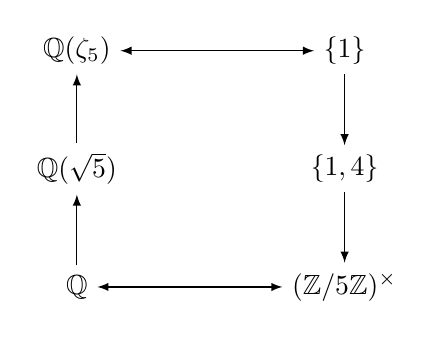
\begin{tikzpicture}[>=latex]
  \node (a) at (0,3.0) {$\mathbb{Q}(\zeta_{5})$};
  \node (b) at (0,1.5) {$\mathbb{Q}(\sqrt 5)$};
  \node (c) at (0,0)   {$\mathbb{Q}$};
  \node (x) at (3.4,3.0) {$\{ 1 \}$};
  \node (y) at (3.4,1.5) {$\{ 1, 4 \}$};
  \node (z) at (3.4,0)   {$(\mathbb{Z}/5\mathbb{Z})^\times$};
  \draw[->] (b) -- (a);
  \draw[->] (c) -- (b);
  \draw[->] (x) -- (y);
  \draw[->] (y) -- (z);
  \draw[<->] (a) -- (x);
  \draw[<->] (c) -- (z);
\end{tikzpicture}
\end{document}
